\documentclass[13pt]{article}

\usepackage{siunitx} % typesets numbers with units very nicely
\usepackage{enumerate} % allows us to customize our lists
\usepackage[brazilian]{babel}
\usepackage[utf8]{inputenc}
\usepackage[T1]{fontenc}
\usepackage{graphicx}

\begin{document}

\title{Sistema de Auxilio de localização de usuários com Tecnologia Indoor Wireless Navigation}
\author{Bruna de Sá Tavares, José Lucas Araújo, Wilton Sapia Dantas}
\date{\today}
\maketitle  

\section*{Introdução}
	Shoppings, convenções,  grandes eventos. Todas esses itens tem o seguinte em comum : São locais internos com uma grande área  que dificulta o senso de localização das pessoas que os frequentam.  Diversas tentativas para resolver este problema foram propostas , desde mapas impressos até totens com mapas eletrônicos . Contudo, nenhuma das soluções atuais possui uma grande praticidade , seja pela necessidade de se encontrar os locais corretos no caso dos totens, seja pela facilidade de perda no caso dos mapas impressos. Nosso projeto visa , além de resolver o problema de localização , gerar um produto pratico e de fácil acesso para todos. Um aplicativo de navegação interna que irá localizar o usuário no local, além de gerar uma rota para algum ponto que o usuário deseja ir.

\section*{Escopo}
	\begin{figure}[!htb]
		\centering
		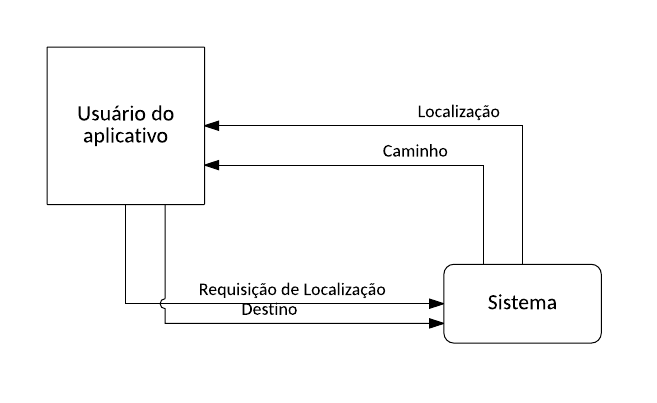
\includegraphics{diagramaContexto.PNG}
		\caption{Diagrama de Contexto}
		O projeto será dividido em dois módulos: o aplicativo android e o servidor.Estes estarão relacionados através da internet.
		\end{figure}
\\
\\
\section*{Oportunidades de Negócio}
	Esse projeto tem como oportunidade de negócio o mapeamento de eventos, locais públicos como: shoppings, aeroportos e terminais de viação.

\section*{Descrição dos Stakeholders}
	-Instituto Mauá de Tecnologia \\
	-Funcionários \\
	-Alunos \\
	-Visitantes \\
	-Administradores(nós)\\
	-Linktel \\
	-Evento Eureka \\
	-Evento Mauá Hand-On \\
	-Semana de Engenharia \\
	-iDocent (projeto de referência) \\ 
	
\section*{Ambiente atual do cliente}
\section*{Módulos do Sistema}
\section*{Precedência e Prioridades}
\section*{Requisitos Funcionais}
\section*{Requitos Não Funcionais}
\section*{Restrições}
\section*{Ambiente Operacional}
Java Android, SqLite, MySql, PHP, Apache server, HTML/CSS, Javascript, Ajax.
\section*{Visão Geral do Sistema - Modelo Conceitual}
\section*{Glossário}

\section*{Referências}

 \end{document}